\documentclass[../../topologia_algebraica]{subfiles}
\begin{document}
\section{La ley exponencial y la suspensi\'on reducida}

En la categor\'ia de conjuntos se cumple que:

\import{\directory}{ejercicios/7} %%%%%%%%%%%%%%%%%%%%%%%%%%%%%%%%%%%%%%%%%%%%%%%%%%%% EJERCICIO 7

En la categor\'ia $\mathbf{Top}$ si sustituimos $\Hom{\cdot,\cdot}$ por $\text{Map}(\cdot,\cdot)$
entonces
\begin{equation}\label{eq:ley_exp_mapeos_continuos}
  \Phi: \text{Map}(X\times Z,Y) \lra \text{Map}(X,\text{Map}(Z\times Y))
\end{equation}
no es necesariamente una biyecci\'on porque la imagen de alguna $f\in\text{Map}(X\times Z,Y)$
bajo $\Phi$ no necesariamente es continua. Pero si le pedimos propiedades adicionales a $Z$
podemos hacer que $\Phi$ sea biyectiva:

\begin{thm}
  Si $Z$ es localmente compacto y Hausdorff, entonces $\Phi$ de (\ref{eq:ley_exp_mapeos_continuos})
  es biyectiva.
\end{thm}

Para este caso particular vamos a hacer $Z=I$ que claramente es localmente compacto (pues es compacto)
y Hausdorff, entonces el teorema es v\'alido. Adem\'as, si quiero aplicarlo a lazos y al grupo
fundamental, es necesario cambiar de categor\'ia a $\mathbf{Top}_*$ e identificar $I\ra I/\partial I$.
El lado derecho de \ref{eq:ley_exp_mapeos_continuos} es f\'acil cambiarlo pero no es inmediatamente
obvio que es lo hay que hacer del lado izquierdo para mantener la biyecci\'on:
\[
  \begin{tikzcd}
    \text{Map}(X\times I,Y) \arrow[r,"\Phi"] \arrow[d,squiggly] &
    \text{Map}(X,\text{Map}(I,Y)) \arrow[d,squiggly] \\
    \text{?} \arrow[r,leftrightarrow] & \text{Map}_*((X,x_0),\Omega(Y,y_0))
  \end{tikzcd}
\]

Considera $f\in\text{Map}(X\times I,Y)$ arbitrario. Quiero que $\Phi_f(x)\in\Omega(Y,y_0)$, es decir
$\Phi_f(x)(0)=f(x,0)=y_0=f(x,1)=\Phi_f(x)(1)$ para toda $x\in X$. Una forma de forzar esto es
identificar, en $X\times I$, todos los puntos de la forma $(x,0)$ \'o $(x,1)$. Entonces el primer paso
es hacer:
\[
  \begin{tikzcd}
      X\times I \arrow[r,squiggly] & X\times I/_{(X\times\{0\})\cup(X\times \{1\})}
  \end{tikzcd}
\]

Tambi\'en quiero que $\Phi_f$ sea un morfismo de espacios basados, es decir que $\Phi_f(x_0)$ es el
punto base de $\Omega(Y,y_0)$, ie. el lazo contante $e_{y_0}$. Esto significa que
$\Phi_f(x_0)(t)=e_{y_0}(t)=y_0$ para toda $t\in I$. Similarmente fuerzo esta condici\'on al identificar
todo el conjunto $\{x_0\}\times I$ en $X\times I$:
\[
  \begin{tikzcd}
    X\times I \arrow[r,squiggly] &
    X\times I/_{(X\times\{0\})\cup(X\times \{1\})} \arrow[r,squiggly] &
    X\times I/_{(X\times\{0\})\cup(X\times \{1\})\cup(\{x_0\}\times I)}.
  \end{tikzcd}
\]

Resulta que esto es suficiente para traducir la biyecci\'on $\Phi$ de (\ref{eq:ley_exp_mapeos_continuos})
al espacio de lazos. La contrucci\'on anterior tiene un nombre:

\begin{defin}
  Sea $(X,x_0)$ un espacio basado, entonces la \emph{suspensi\'on reducida} de $X$ es:
  \[
    \Ss X:=(X\times I)/_{(X\times\{0\})\cup(X\times \{1\})\cup(\{x_0\}\times I)}
  \]
  y tambi\'en es un espacio basado con base $\star$, el punto al que se identifica todo el
  conjunto $(X\times\{0\})\cup(X\times \{1\})\cup(\{x_0\}\times I)$.
\end{defin}

\begin{nota}
  A veces es \'util definir el paso intermedio que se us\'o para definir la suspensi\'on
  reducida. Si defino $A=X\times\{0\}\subset X\times I$ y $B=X\times\{1\}\subset X\times I$,
  entonces la \emph{suspensi\'on no-reducida} de $X$ es el cociente:
  \[
    \Sigma X := (X\times I)/_{A,B}.
  \]
  Observa que no estoy identificando $A\cup B$ a un punto. M\'as bien estoy identificando $A$
  a un punto y $B$ a otro punto. La figura%
%%%%%%%%%%%%%%%%%%%%%%%%%%%%%%%%%%%%%%%%%%%%%%%%%%%%%%%%%%%%%%%%%%%%% FIGURA % SUSPENSION CIRCULO
  \begin{figure}
    \centering
    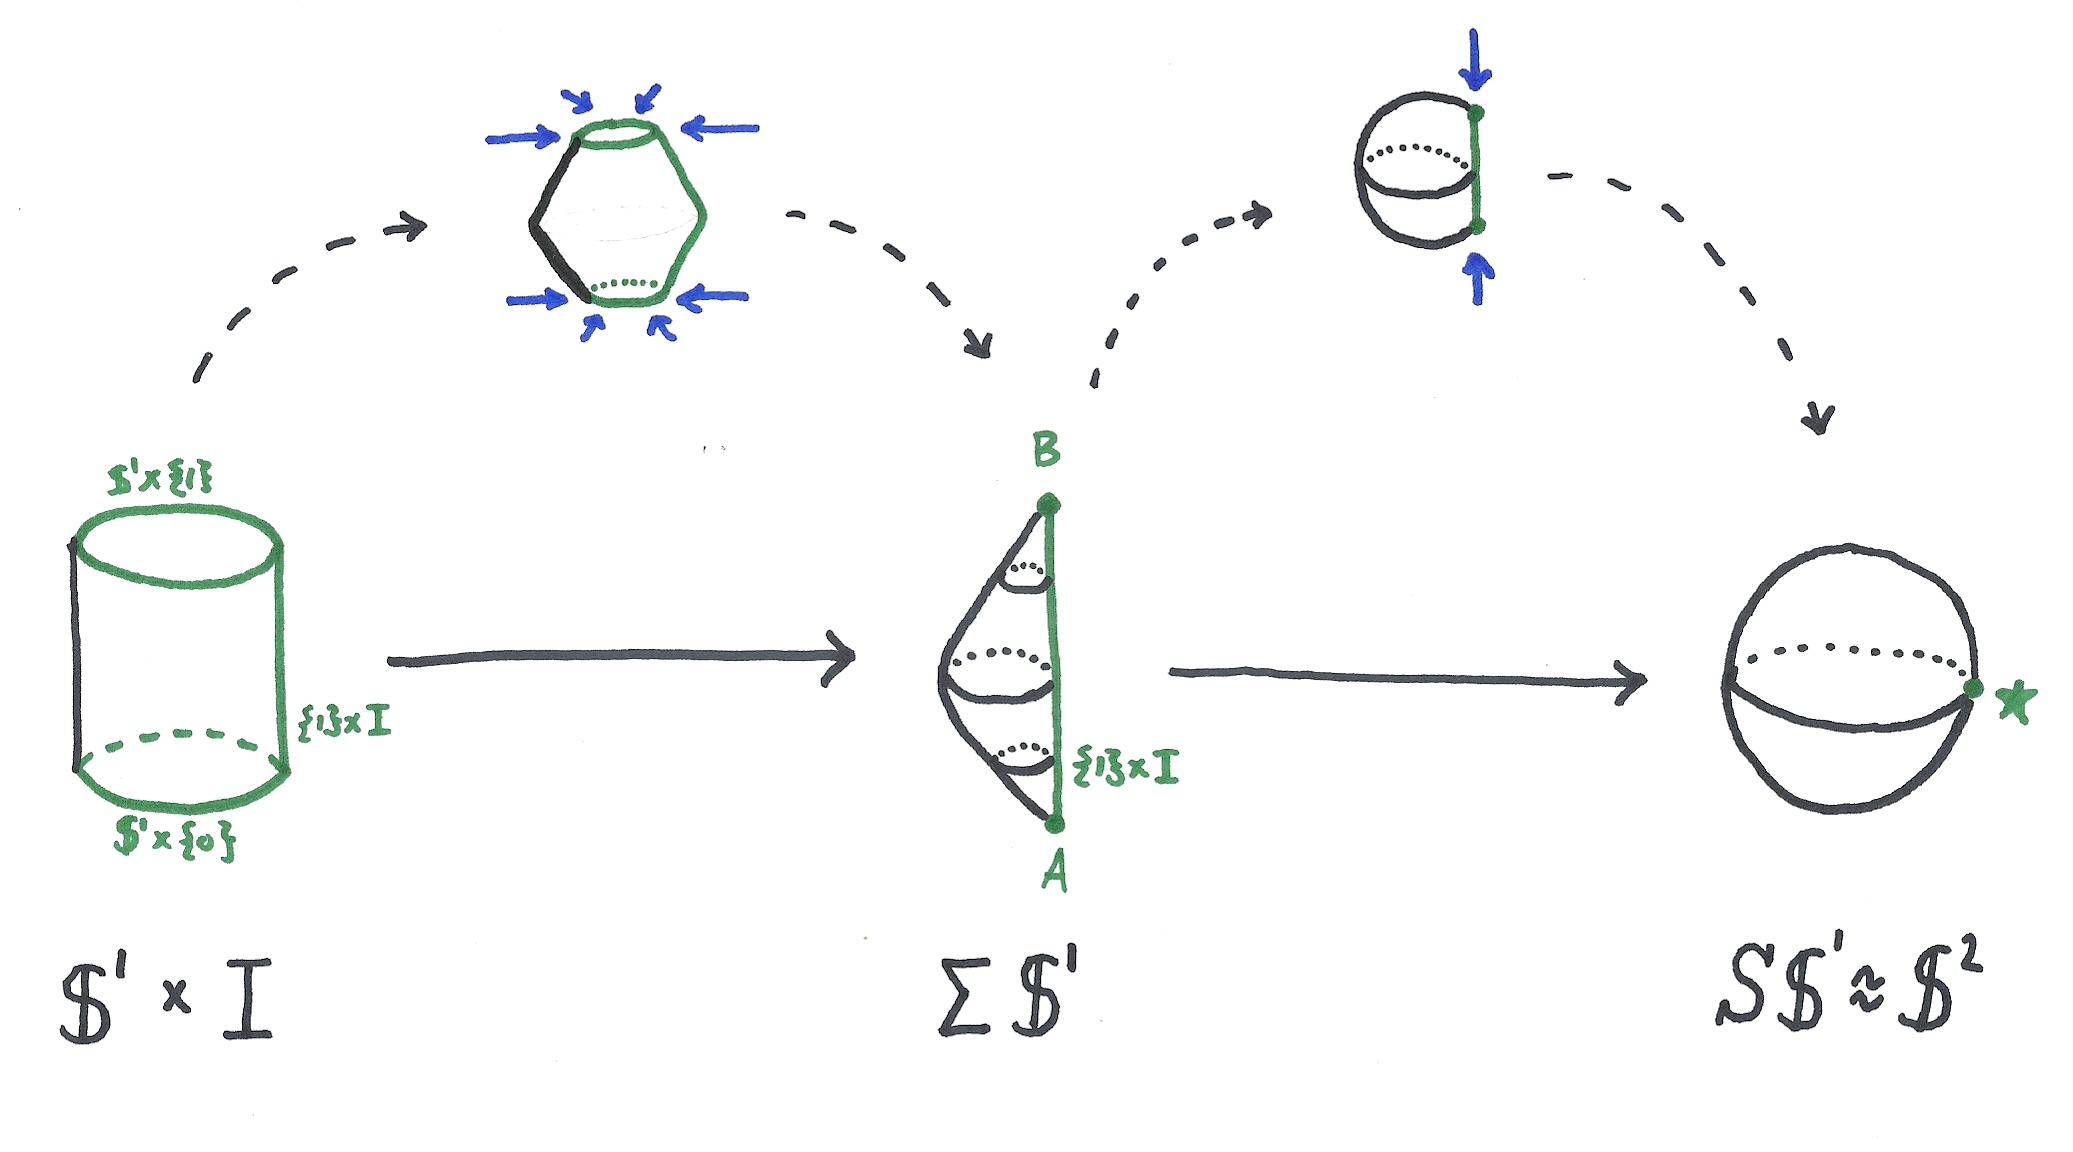
\includegraphics[scale=0.18]{suspension_circulo}
    \caption{Construcci\'on de $\Ss\Sn^1$.}
    \label{fig:suspension_circulo}
  \end{figure}
%%%%%%%%%%%%%%%%%%%%%%%%%%%%%%%%%%%%%%%%%%%%%%%%%%%%%%%%%%%%%%%%%%%%%%%%%%%%%%%%%%%%%%%%%%%%%%%%
  \ref{fig:suspension_circulo} ilustra los pasos para construir la suspensi\'on de $\Sn^1$.

  Vale la pena mencionar que la figura \ref{fig:suspension_circulo} tambi\'en funciona
  para visualizar la construcci\'on de la suspensi\'on reducida del disco; el cilindro
  del inicio est\'a relleno en este caso y por lo tanto la esfera al final est\'a rellena
  tambi\'en, por lo tanto $\Ss\mathbb{D}^2\approx B_1(0)\subset\RR^3$ la bola de radio 1
  con centro en el origen.
\end{nota}

Con esta definici\'on, puedo reescribir (\ref{eq:ley_exp_mapeos_continuos}) como:

\import{\directory}{ejercicios/8}  %%%%%%%%%%%%%%%%%%%%%%%%%%%%%%%%%%%%%%%%%%%%%%%%% EJERCICIO 8

La suspensi\'on reducida es un funtor
$\Ss:\mathbf{Top}_*\ra\mathbf{Top}_*$. En efecto, si $f:(X,x_0)\ra (Y,y_0)$ es un morfismo,
entonces la funci\'on continua $(f\times\Id_I):X\times I \ra Y\times I$ se factoriza a trav\'es
de $\Ss X$, es decir:
\[
  \begin{tikzcd}
    X\times I \arrow[rr,"f\times\Id_I"] \arrow[d,twoheadrightarrow] & &
    Y\times I \arrow[d,twoheadrightarrow]\\
    \Ss X \arrow[rr,dashed,"\Ss f"] & & \Ss Y
  \end{tikzcd}
\]
Esto sucede porque
\[
  (f\times\Id_I)(x,0)=(f(x),0)\; ,\quad (f\times\Id_I)(x,1)=(f(x),1)\; ,\quad
  (f\times\Id_I)(x_o,t)=(y_0,t) \qquad\forall x\in X, \; t\in I,
\]
es decir que el conjunto en $X\times I$ que se identifica a un punto se manda, bajo $f\times\Id_I$,
al conjunto de $Y\times I$ que se identifica a un punto.

Adem\'as claramente tengo que $\Ss\Id_X=\Id_{\Ss X}$ porque $\Ss\Id_X$ es inducido por
$\Id_X\times\Id_I=\Id_{X\times I}$ y por \'ultimo, si $(X,x_0)\morf{f}(Y,y_0)\morf{g}(Z,z_0)$,
entonces $(g\circ f)\times\Id_I=(g\times\Id_I)\circ(f\times\Id_I)$ y as\'i
$\Ss(g\circ f)=\Ss g\circ\Ss f$. Por lo tanto he probado que:

\begin{prop}
  La suspensi\'on reducida es un funtor (covariante) $\Ss:\mathbf{Top}_*\ra\mathbf{Top}_*$.
\end{prop}

Podemos juntar esta proposici\'on con la proposici\'on \ref{prop:omega_funtor} y el ejercicio
\ref{ej:ocho} para deducir:

\begin{cor}
  Los funtores $\Ss:\mathbf{Top}_*\ra\mathbf{Top}_*$ y $\Omega:\mathbf{Top}_*\ra\mathbf{Top}_*$
  son funtores adjuntos, m\'as precisamente $\Ss$ es adjunto izquierdo de $\Omega$ y $\Omega$ es
  adjunto derecho de $\Ss$:
  \[
    \text{Hom}(\Ss X,Y) \longleftrightarrow \text{Hom}(X,\Omega Y)
  \]
  donde he sustituido $\text{Map}_*(\cdot,\cdot)$ por la notaci\'on categ\'orica.
\end{cor}

M\'as que $\text{Map}_*$, me interesa las clases de equivalencia m\'odulo homotop\'ia.
Resulta que la funci\'on $\Phi$ del ejercicio \ref{ej:ocho} se factoriza a trav\'es de
las clases de homotop\'ia. M\'as precisamente:

\import{\directory}{ejercicios/11} %%%%%%%%%%%%%%%%%%%%%%%%%%%%%%%%%%%%%%%%%%%%%%%%%%% EJERCICIO 11

Intuitivamente, el ejercicio \ref{ej:11} dice que la propiedad adjunta de los funtores
$\Ss$ y $\Omega$ se preserva bajo homotop\'ias.
\end{document}